% Light: latex architecture.tex && dvisvgm --no-fonts architecture.dvi -o architecture-light.svg
% Dark:  latex '\def\darkmode{1}% Light: latex architecture.tex && dvisvgm --no-fonts architecture.dvi -o architecture-light.svg
% Dark:  latex '\def\darkmode{1}% Light: latex architecture.tex && dvisvgm --no-fonts architecture.dvi -o architecture-light.svg
% Dark:  latex '\def\darkmode{1}% Light: latex architecture.tex && dvisvgm --no-fonts architecture.dvi -o architecture-light.svg
% Dark:  latex '\def\darkmode{1}\input{architecture.tex}' && dvisvgm --no-fonts architecture.dvi -o architecture-dark.svg
\documentclass[tikz,border=32pt]{standalone}
\usepackage[T1]{fontenc}
\usepackage{lmodern}
\usepackage{xcolor}
\usetikzlibrary{positioning,fit,backgrounds,arrows.meta,calc}

\ifdefined\darkmode
  \definecolor{jafillblue}{RGB}{23,31,46}
  \definecolor{jafilltools}{RGB}{29,39,58}
  \definecolor{jafillamber}{RGB}{38,30,20}
  \definecolor{jafillpurple}{RGB}{32,26,46}
  \definecolor{jagroup}{RGB}{100,116,139}
  \definecolor{jaarrow}{RGB}{148,163,184}
  \definecolor{jadatabg}{RGB}{6,78,59}
  \definecolor{jadatatext}{RGB}{167,243,208}
  \definecolor{jasub}{RGB}{148,163,184}
  \definecolor{jalabelbg}{RGB}{30,41,59}
\else
  \definecolor{jafillblue}{RGB}{244,247,253}
  \definecolor{jafilltools}{RGB}{234,241,251}
  \definecolor{jafillamber}{RGB}{253,248,240}
  \definecolor{jafillpurple}{RGB}{248,245,253}
  \definecolor{jagroup}{RGB}{148,163,184}
  \definecolor{jaarrow}{RGB}{100,116,139}
  \definecolor{jadatabg}{RGB}{236,253,245}
  \definecolor{jadatatext}{RGB}{6,95,70}
  \definecolor{jasub}{RGB}{100,116,139}
  \definecolor{jalabelbg}{RGB}{255,255,255}
\fi

\definecolor{japython}{RGB}{37,99,235}
\definecolor{japythonstroke}{RGB}{30,64,175}
\definecolor{jajulia}{RGB}{124,58,237}
\definecolor{jajuliastroke}{RGB}{91,33,182}
\definecolor{jastorage}{RGB}{180,83,9}
\definecolor{jastoragestroke}{RGB}{146,64,14}
\definecolor{jadata}{RGB}{4,120,87}
\definecolor{jadatastroke}{RGB}{6,95,70}
\definecolor{jaexternal}{RGB}{71,85,105}
\definecolor{jaexternalstroke}{RGB}{51,65,85}

\tikzset{
  base/.style={
    draw, rounded corners=2pt, font=\small\sffamily,
    align=center, inner sep=6pt, minimum height=9mm, text=white
  },
  python/.style={base, fill=japython, draw=japythonstroke},
  julia/.style={base, fill=jajulia, draw=jajuliastroke},
  storage/.style={base, fill=jastorage, draw=jastoragestroke, font=\footnotesize\sffamily},
  external/.style={base, fill=jaexternal, draw=jaexternalstroke},
  data/.style={
    draw=jadatastroke, rounded corners=2pt, fill=jadatabg,
    font=\footnotesize\sffamily, align=left, inner sep=7pt, text=jadatatext
  },
  grouplabel/.style={font=\footnotesize\sffamily, text=jagroup},
  bi/.style={
    {Stealth[length=2mm,width=1.6mm]}-{Stealth[length=2mm,width=1.6mm]},
    draw=jaarrow, semithick
  },
  ar/.style={-{Stealth[length=2.2mm,width=1.8mm]}, draw=jaarrow, semithick},
  ard/.style={-{Stealth[length=2.2mm,width=1.8mm]}, draw=jadata, semithick, dashed},
  el/.style={font=\footnotesize\sffamily, text=jasub, fill=jalabelbg, inner sep=2pt},
}

\begin{document}
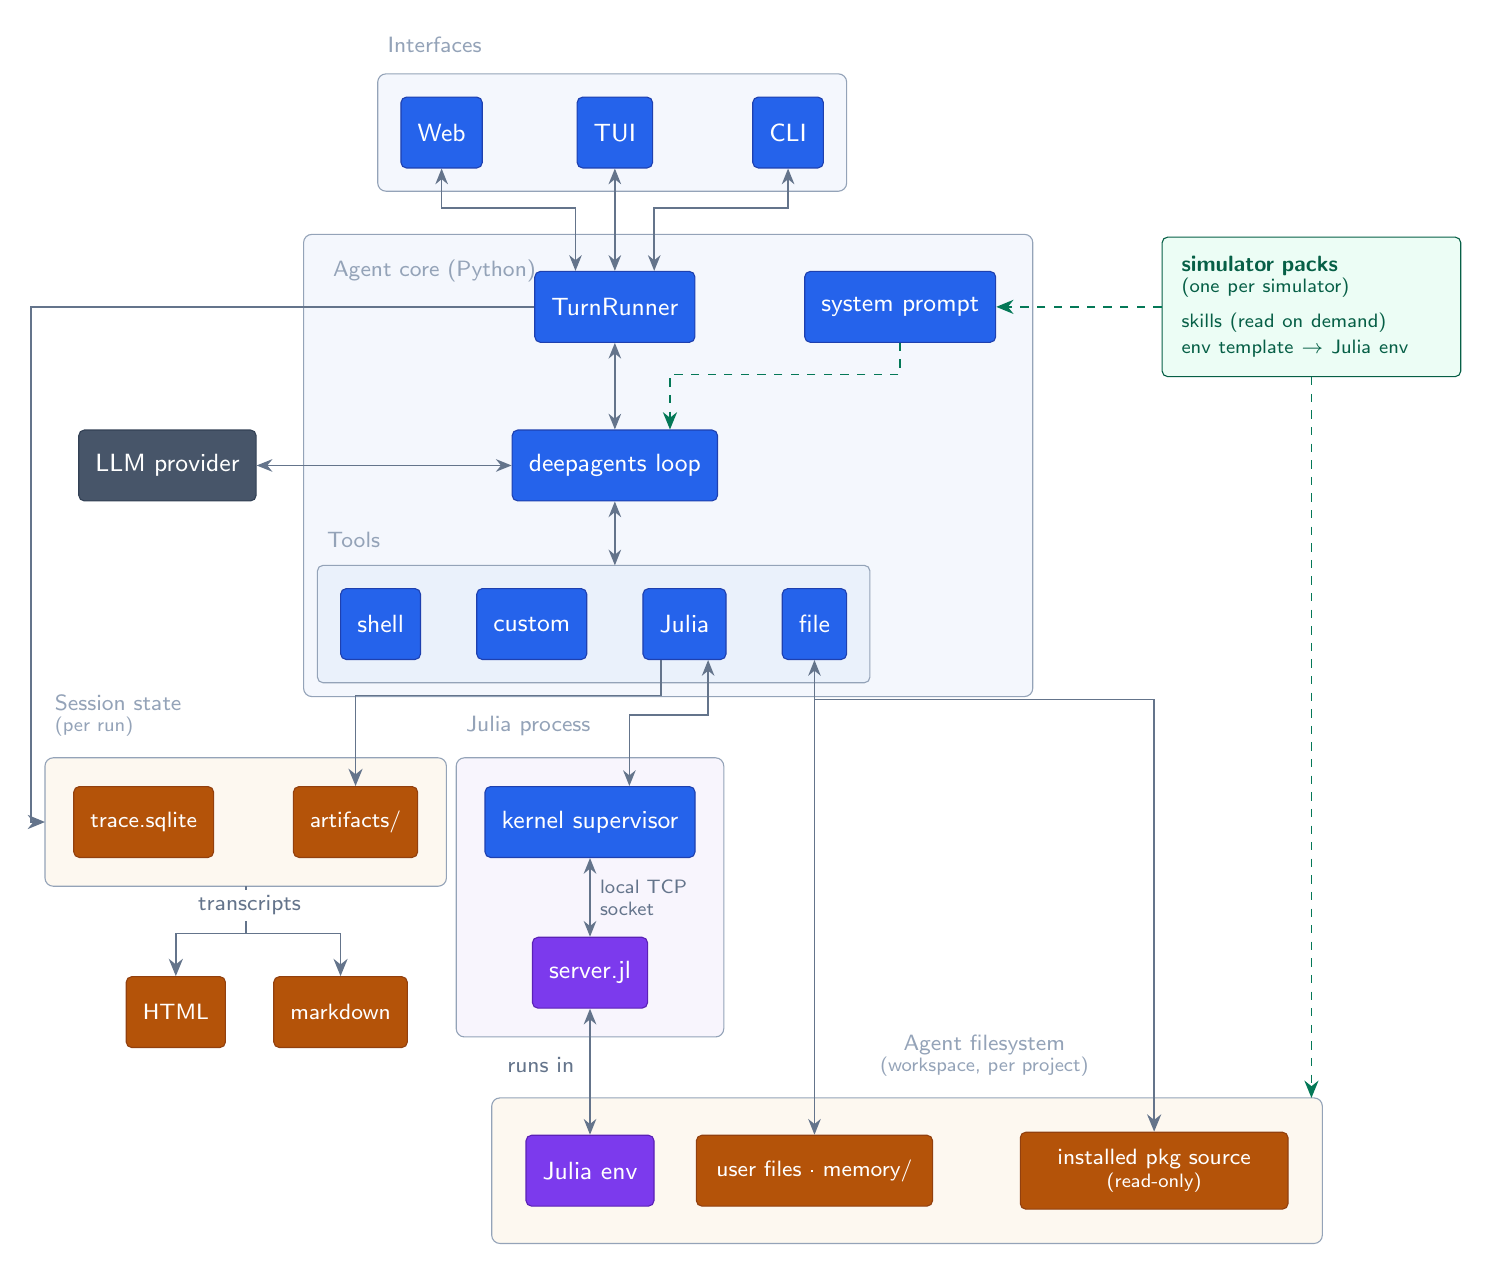
\begin{tikzpicture}

  % ===== agent core spine, interfaces centred over the TurnRunner =====
  \node[python] (runner) {TurnRunner};
  \node[python, anchor=south] (web) at ([xshift=-22mm,yshift=13mm]runner.north) {Web};
  \node[python, anchor=south] (tui) at ([yshift=13mm]runner.north) {TUI};
  \node[python, anchor=south] (cli) at ([xshift=22mm,yshift=13mm]runner.north) {CLI};

  \node[python, below=11mm of runner] (loop) {deepagents loop};

  % tools row, centred under the loop
  \node[python, anchor=north east] (ct) at ([xshift=-3.5mm,yshift=-11mm]loop.south) {custom};
  \node[python, left=7mm of ct] (sh) {shell};
  \node[python, anchor=north west] (jt) at ([xshift=3.5mm,yshift=-11mm]loop.south) {Julia};
  \node[python, right=7mm of jt] (ft) {file};

  % ===== prompt inside the core, packs beside it, LLM on the left =====
  \node[python] (prompt) at ([xshift=26mm]runner.east |- runner) {system prompt};
  \node[external, anchor=east] (llm) at ([xshift=-10.6mm]sh.west |- loop) {LLM provider};
  \node[data, anchor=west, text width=33mm] (pack) at ([xshift=21mm]prompt.east) {%
    \textbf{simulator packs}\\[-2pt]
    {\scriptsize (one per simulator)}\\[3pt]
    {\scriptsize skills (read on demand)}\\
    {\scriptsize env template $\rightarrow$ Julia env}};

  % ===== left column: session state =====
  \node[storage, below left=16mm and 16mm of sh] (trace) {trace.sqlite};
  \node[storage, right=10mm of trace] (arts) {artifacts/};
  \coordinate (sessmid) at ($(trace.south)!0.5!(arts.south)$);
  \node[storage, anchor=north east] (html) at ([xshift=-3mm,yshift=-15mm]sessmid) {HTML};
  \node[storage, anchor=north west] (md) at ([xshift=3mm,yshift=-15mm]sessmid) {markdown};

  % ===== julia process column, left of the file-tool feed =====
  \node[python, below=16mm of jt, xshift=-12mm] (kern) {kernel supervisor};
  \node[julia, below=10mm of kern] (serv) {server.jl};

  % ===== bottom: filesystem; env straight under the server =====
  \node[julia, anchor=north] (env) at ([yshift=-16mm]serv.south) {Julia env};
  \node[storage, minimum width=30mm] (files) at (ft |- env) {user files · memory/};
  \node[storage, right=11mm of files, minimum width=34mm] (mounts) {%
    installed pkg source\\[-1pt]
    {\scriptsize (read-only)}};

  % ===== group boxes =====
  \begin{scope}[on background layer]
    \node[fit=(web)(tui)(cli), inner sep=8pt] (ifacebox) {};
    \draw[jagroup, fill=jafillblue, rounded corners=3pt] (ifacebox.south west) rectangle (ifacebox.north east);
    \node[grouplabel, anchor=south west] at ([yshift=1.5mm]ifacebox.north west) {Interfaces};

    \node[fit=(runner)(loop)(sh)(ct)(jt)(ft)(prompt), inner sep=13pt] (corebox) {};
    \draw[jagroup, fill=jafillblue, rounded corners=3pt] (corebox.south west) rectangle (corebox.north east);
    \node[grouplabel, anchor=north west] at ([xshift=2.5mm,yshift=-2mm]corebox.north west) {Agent core (Python)};

    \node[fit=(sh)(ct)(jt)(ft), inner sep=8pt] (toolsbox) {};
    \draw[jagroup, fill=jafilltools, rounded corners=2pt] (toolsbox.south west) rectangle (toolsbox.north east);
    \node[grouplabel, anchor=south west] at ([yshift=1mm]toolsbox.north west) {Tools};

    \node[fit=(trace)(arts), inner sep=10pt] (sessbox) {};
    \draw[jagroup, fill=jafillamber, rounded corners=3pt] (sessbox.south west) rectangle (sessbox.north east);
    \node[grouplabel, anchor=south west, align=left] at ([yshift=1.5mm]sessbox.north west)
      {Session state\\[-2pt]{\scriptsize (per run)}};

    \node[fit=(kern)(serv), inner sep=10pt] (jlbox) {};
    \draw[jagroup, fill=jafillpurple, rounded corners=3pt] (jlbox.south west) rectangle (jlbox.north east);
    \node[grouplabel, anchor=south west] at ([yshift=1.5mm]jlbox.north west) {Julia process};

    \node[fit=(env)(files)(mounts), inner sep=12pt] (fsbox) {};
    \draw[jagroup, fill=jafillamber, rounded corners=3pt] (fsbox.south west) rectangle (fsbox.north east);
    \coordinate (fslabelx) at ($(files.north)!0.5!(mounts.north)$);
    \node[grouplabel, anchor=south, align=center] at ([yshift=1.5mm]fslabelx |- fsbox.north)
      {Agent filesystem\\[-2pt]{\scriptsize (workspace, per project)}};
  \end{scope}

  % ===== edges =====
  \draw[bi] (web.south) -- ++(0,-5mm) -| ([xshift=-5mm]runner.north);
  \draw[bi] (tui.south) -- ++(0,-5mm) -| (runner.north);
  \draw[bi] (cli.south) -- ++(0,-5mm) -| ([xshift=5mm]runner.north);
  \draw[bi] (runner.south) -- (loop.north);
  \draw[ard] (pack.west) -- (prompt.east);
  \draw[ard] (pack.south) -- (pack.south |- fsbox.north);
  \draw[ard] (prompt.south) -- ++(0,-4mm) -| ([xshift=7mm]loop.north);
  \draw[bi] (llm.east) -- (loop.west);
  \draw[bi] (loop.south) -- (loop.south |- toolsbox.north);

  % TurnRunner -> session state, dropping left of the LLM provider
  \coordinate (leftbus) at ($(llm.west)+(-6mm,0)$);
  \draw[ar] (runner.west) -- (leftbus |- runner.west) -- (leftbus |- sessbox.west) -- (sessbox.west);
  \draw[ar] (sessbox.south) -- ++(0,-6mm) -| (html.north);
  \draw[ar] (sessbox.south) -- ++(0,-6mm) -| (md.north);
  \node[el] at ([yshift=-6mm]sessmid) {transcripts};

  % julia spine and artifacts, on separate bands so nothing crosses
  \draw[bi] ([xshift=3mm]jt.south) -- ++(0,-7mm) -| ([xshift=5mm]kern.north);
  \draw[ar] ([xshift=-3mm]jt.south) -- ++(0,-4.5mm) -| (arts.north);
  \draw[bi] (kern.south) -- node[right, align=left, font=\scriptsize\sffamily, text=jasub] {local TCP\\socket} (serv.north);
  \draw[bi] (serv.south) -- node[el, left=1.2mm, pos=0.45] {runs in} (env.north);

  % file tool -> workspace nodes
  \draw[bi] (ft.south) -- (files.north);
  \draw[ar] ([yshift=-5mm]ft.south) -| (mounts.north);

\end{tikzpicture}
\end{document}
' && dvisvgm --no-fonts architecture.dvi -o architecture-dark.svg
\documentclass[tikz,border=32pt]{standalone}
\usepackage[T1]{fontenc}
\usepackage{lmodern}
\usepackage{xcolor}
\usetikzlibrary{positioning,fit,backgrounds,arrows.meta,calc}

\ifdefined\darkmode
  \definecolor{jafillblue}{RGB}{23,31,46}
  \definecolor{jafilltools}{RGB}{29,39,58}
  \definecolor{jafillamber}{RGB}{38,30,20}
  \definecolor{jafillpurple}{RGB}{32,26,46}
  \definecolor{jagroup}{RGB}{100,116,139}
  \definecolor{jaarrow}{RGB}{148,163,184}
  \definecolor{jadatabg}{RGB}{6,78,59}
  \definecolor{jadatatext}{RGB}{167,243,208}
  \definecolor{jasub}{RGB}{148,163,184}
  \definecolor{jalabelbg}{RGB}{30,41,59}
\else
  \definecolor{jafillblue}{RGB}{244,247,253}
  \definecolor{jafilltools}{RGB}{234,241,251}
  \definecolor{jafillamber}{RGB}{253,248,240}
  \definecolor{jafillpurple}{RGB}{248,245,253}
  \definecolor{jagroup}{RGB}{148,163,184}
  \definecolor{jaarrow}{RGB}{100,116,139}
  \definecolor{jadatabg}{RGB}{236,253,245}
  \definecolor{jadatatext}{RGB}{6,95,70}
  \definecolor{jasub}{RGB}{100,116,139}
  \definecolor{jalabelbg}{RGB}{255,255,255}
\fi

\definecolor{japython}{RGB}{37,99,235}
\definecolor{japythonstroke}{RGB}{30,64,175}
\definecolor{jajulia}{RGB}{124,58,237}
\definecolor{jajuliastroke}{RGB}{91,33,182}
\definecolor{jastorage}{RGB}{180,83,9}
\definecolor{jastoragestroke}{RGB}{146,64,14}
\definecolor{jadata}{RGB}{4,120,87}
\definecolor{jadatastroke}{RGB}{6,95,70}
\definecolor{jaexternal}{RGB}{71,85,105}
\definecolor{jaexternalstroke}{RGB}{51,65,85}

\tikzset{
  base/.style={
    draw, rounded corners=2pt, font=\small\sffamily,
    align=center, inner sep=6pt, minimum height=9mm, text=white
  },
  python/.style={base, fill=japython, draw=japythonstroke},
  julia/.style={base, fill=jajulia, draw=jajuliastroke},
  storage/.style={base, fill=jastorage, draw=jastoragestroke, font=\footnotesize\sffamily},
  external/.style={base, fill=jaexternal, draw=jaexternalstroke},
  data/.style={
    draw=jadatastroke, rounded corners=2pt, fill=jadatabg,
    font=\footnotesize\sffamily, align=left, inner sep=7pt, text=jadatatext
  },
  grouplabel/.style={font=\footnotesize\sffamily, text=jagroup},
  bi/.style={
    {Stealth[length=2mm,width=1.6mm]}-{Stealth[length=2mm,width=1.6mm]},
    draw=jaarrow, semithick
  },
  ar/.style={-{Stealth[length=2.2mm,width=1.8mm]}, draw=jaarrow, semithick},
  ard/.style={-{Stealth[length=2.2mm,width=1.8mm]}, draw=jadata, semithick, dashed},
  el/.style={font=\footnotesize\sffamily, text=jasub, fill=jalabelbg, inner sep=2pt},
}

\begin{document}
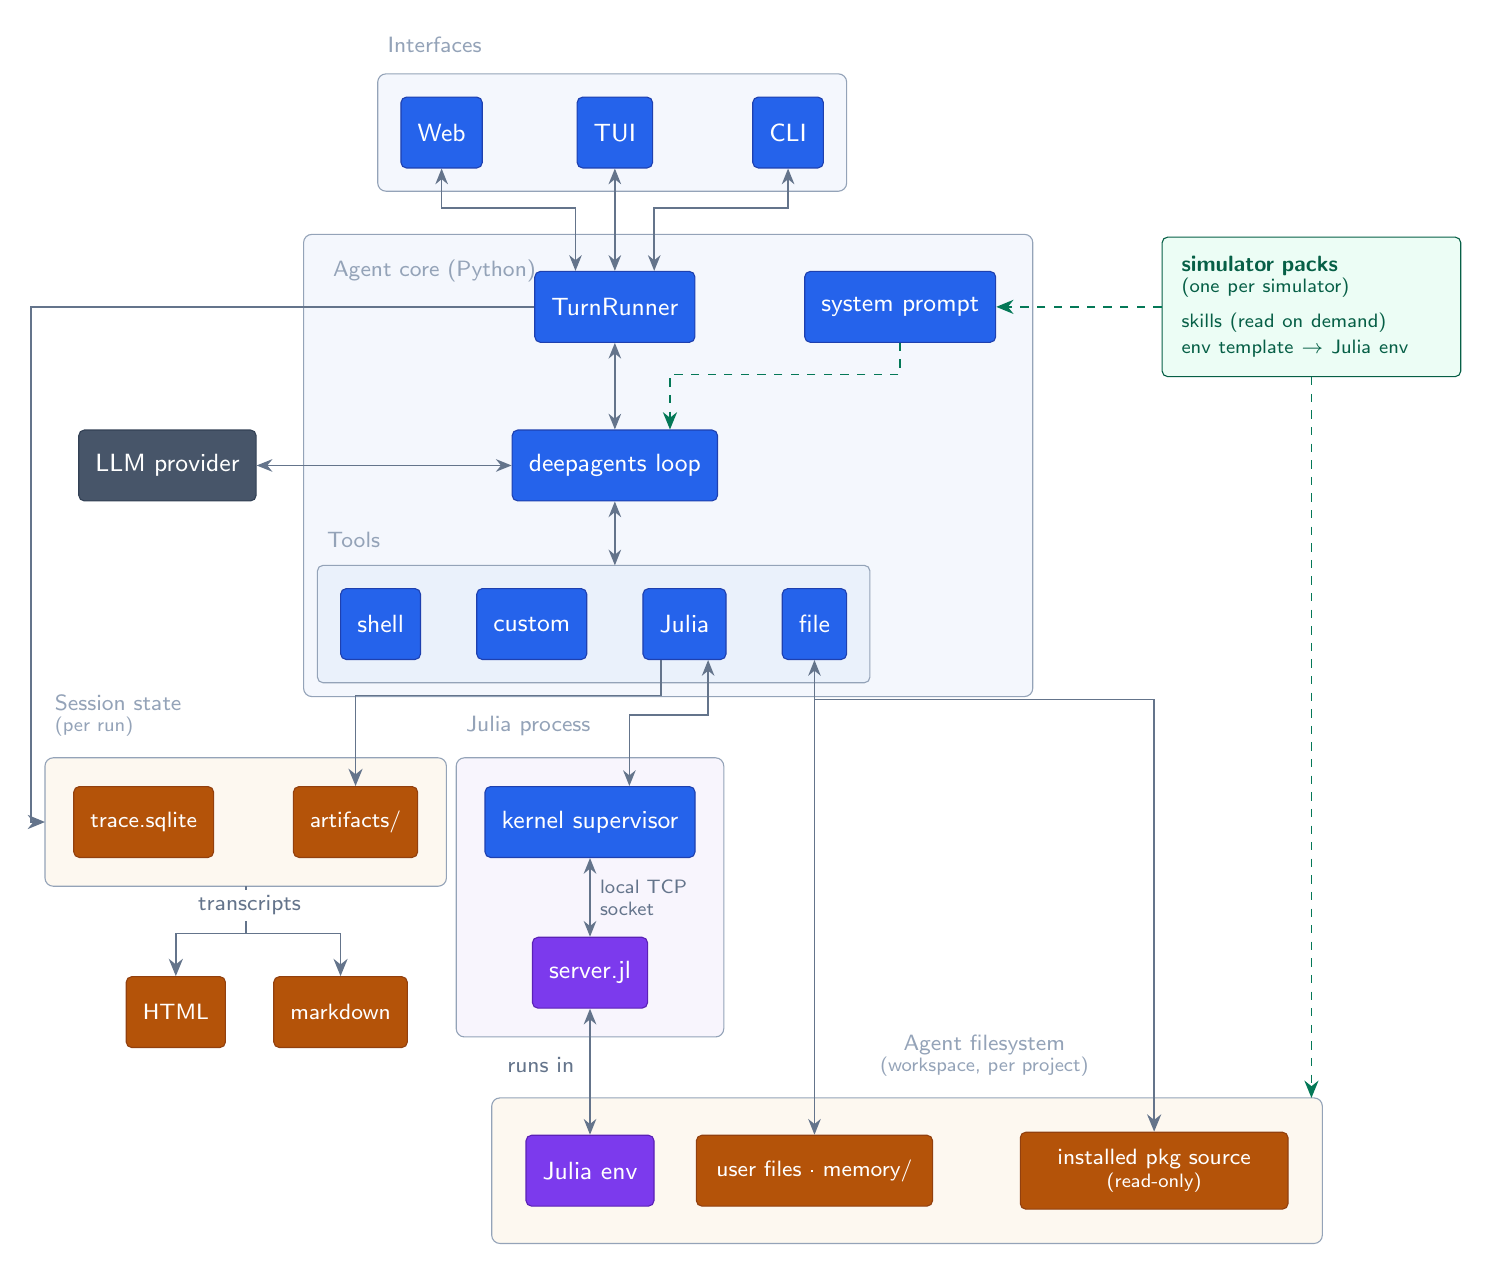
\begin{tikzpicture}

  % ===== agent core spine, interfaces centred over the TurnRunner =====
  \node[python] (runner) {TurnRunner};
  \node[python, anchor=south] (web) at ([xshift=-22mm,yshift=13mm]runner.north) {Web};
  \node[python, anchor=south] (tui) at ([yshift=13mm]runner.north) {TUI};
  \node[python, anchor=south] (cli) at ([xshift=22mm,yshift=13mm]runner.north) {CLI};

  \node[python, below=11mm of runner] (loop) {deepagents loop};

  % tools row, centred under the loop
  \node[python, anchor=north east] (ct) at ([xshift=-3.5mm,yshift=-11mm]loop.south) {custom};
  \node[python, left=7mm of ct] (sh) {shell};
  \node[python, anchor=north west] (jt) at ([xshift=3.5mm,yshift=-11mm]loop.south) {Julia};
  \node[python, right=7mm of jt] (ft) {file};

  % ===== prompt inside the core, packs beside it, LLM on the left =====
  \node[python] (prompt) at ([xshift=26mm]runner.east |- runner) {system prompt};
  \node[external, anchor=east] (llm) at ([xshift=-10.6mm]sh.west |- loop) {LLM provider};
  \node[data, anchor=west, text width=33mm] (pack) at ([xshift=21mm]prompt.east) {%
    \textbf{simulator packs}\\[-2pt]
    {\scriptsize (one per simulator)}\\[3pt]
    {\scriptsize skills (read on demand)}\\
    {\scriptsize env template $\rightarrow$ Julia env}};

  % ===== left column: session state =====
  \node[storage, below left=16mm and 16mm of sh] (trace) {trace.sqlite};
  \node[storage, right=10mm of trace] (arts) {artifacts/};
  \coordinate (sessmid) at ($(trace.south)!0.5!(arts.south)$);
  \node[storage, anchor=north east] (html) at ([xshift=-3mm,yshift=-15mm]sessmid) {HTML};
  \node[storage, anchor=north west] (md) at ([xshift=3mm,yshift=-15mm]sessmid) {markdown};

  % ===== julia process column, left of the file-tool feed =====
  \node[python, below=16mm of jt, xshift=-12mm] (kern) {kernel supervisor};
  \node[julia, below=10mm of kern] (serv) {server.jl};

  % ===== bottom: filesystem; env straight under the server =====
  \node[julia, anchor=north] (env) at ([yshift=-16mm]serv.south) {Julia env};
  \node[storage, minimum width=30mm] (files) at (ft |- env) {user files · memory/};
  \node[storage, right=11mm of files, minimum width=34mm] (mounts) {%
    installed pkg source\\[-1pt]
    {\scriptsize (read-only)}};

  % ===== group boxes =====
  \begin{scope}[on background layer]
    \node[fit=(web)(tui)(cli), inner sep=8pt] (ifacebox) {};
    \draw[jagroup, fill=jafillblue, rounded corners=3pt] (ifacebox.south west) rectangle (ifacebox.north east);
    \node[grouplabel, anchor=south west] at ([yshift=1.5mm]ifacebox.north west) {Interfaces};

    \node[fit=(runner)(loop)(sh)(ct)(jt)(ft)(prompt), inner sep=13pt] (corebox) {};
    \draw[jagroup, fill=jafillblue, rounded corners=3pt] (corebox.south west) rectangle (corebox.north east);
    \node[grouplabel, anchor=north west] at ([xshift=2.5mm,yshift=-2mm]corebox.north west) {Agent core (Python)};

    \node[fit=(sh)(ct)(jt)(ft), inner sep=8pt] (toolsbox) {};
    \draw[jagroup, fill=jafilltools, rounded corners=2pt] (toolsbox.south west) rectangle (toolsbox.north east);
    \node[grouplabel, anchor=south west] at ([yshift=1mm]toolsbox.north west) {Tools};

    \node[fit=(trace)(arts), inner sep=10pt] (sessbox) {};
    \draw[jagroup, fill=jafillamber, rounded corners=3pt] (sessbox.south west) rectangle (sessbox.north east);
    \node[grouplabel, anchor=south west, align=left] at ([yshift=1.5mm]sessbox.north west)
      {Session state\\[-2pt]{\scriptsize (per run)}};

    \node[fit=(kern)(serv), inner sep=10pt] (jlbox) {};
    \draw[jagroup, fill=jafillpurple, rounded corners=3pt] (jlbox.south west) rectangle (jlbox.north east);
    \node[grouplabel, anchor=south west] at ([yshift=1.5mm]jlbox.north west) {Julia process};

    \node[fit=(env)(files)(mounts), inner sep=12pt] (fsbox) {};
    \draw[jagroup, fill=jafillamber, rounded corners=3pt] (fsbox.south west) rectangle (fsbox.north east);
    \coordinate (fslabelx) at ($(files.north)!0.5!(mounts.north)$);
    \node[grouplabel, anchor=south, align=center] at ([yshift=1.5mm]fslabelx |- fsbox.north)
      {Agent filesystem\\[-2pt]{\scriptsize (workspace, per project)}};
  \end{scope}

  % ===== edges =====
  \draw[bi] (web.south) -- ++(0,-5mm) -| ([xshift=-5mm]runner.north);
  \draw[bi] (tui.south) -- ++(0,-5mm) -| (runner.north);
  \draw[bi] (cli.south) -- ++(0,-5mm) -| ([xshift=5mm]runner.north);
  \draw[bi] (runner.south) -- (loop.north);
  \draw[ard] (pack.west) -- (prompt.east);
  \draw[ard] (pack.south) -- (pack.south |- fsbox.north);
  \draw[ard] (prompt.south) -- ++(0,-4mm) -| ([xshift=7mm]loop.north);
  \draw[bi] (llm.east) -- (loop.west);
  \draw[bi] (loop.south) -- (loop.south |- toolsbox.north);

  % TurnRunner -> session state, dropping left of the LLM provider
  \coordinate (leftbus) at ($(llm.west)+(-6mm,0)$);
  \draw[ar] (runner.west) -- (leftbus |- runner.west) -- (leftbus |- sessbox.west) -- (sessbox.west);
  \draw[ar] (sessbox.south) -- ++(0,-6mm) -| (html.north);
  \draw[ar] (sessbox.south) -- ++(0,-6mm) -| (md.north);
  \node[el] at ([yshift=-6mm]sessmid) {transcripts};

  % julia spine and artifacts, on separate bands so nothing crosses
  \draw[bi] ([xshift=3mm]jt.south) -- ++(0,-7mm) -| ([xshift=5mm]kern.north);
  \draw[ar] ([xshift=-3mm]jt.south) -- ++(0,-4.5mm) -| (arts.north);
  \draw[bi] (kern.south) -- node[right, align=left, font=\scriptsize\sffamily, text=jasub] {local TCP\\socket} (serv.north);
  \draw[bi] (serv.south) -- node[el, left=1.2mm, pos=0.45] {runs in} (env.north);

  % file tool -> workspace nodes
  \draw[bi] (ft.south) -- (files.north);
  \draw[ar] ([yshift=-5mm]ft.south) -| (mounts.north);

\end{tikzpicture}
\end{document}
' && dvisvgm --no-fonts architecture.dvi -o architecture-dark.svg
\documentclass[tikz,border=32pt]{standalone}
\usepackage[T1]{fontenc}
\usepackage{lmodern}
\usepackage{xcolor}
\usetikzlibrary{positioning,fit,backgrounds,arrows.meta,calc}

\ifdefined\darkmode
  \definecolor{jafillblue}{RGB}{23,31,46}
  \definecolor{jafilltools}{RGB}{29,39,58}
  \definecolor{jafillamber}{RGB}{38,30,20}
  \definecolor{jafillpurple}{RGB}{32,26,46}
  \definecolor{jagroup}{RGB}{100,116,139}
  \definecolor{jaarrow}{RGB}{148,163,184}
  \definecolor{jadatabg}{RGB}{6,78,59}
  \definecolor{jadatatext}{RGB}{167,243,208}
  \definecolor{jasub}{RGB}{148,163,184}
  \definecolor{jalabelbg}{RGB}{30,41,59}
\else
  \definecolor{jafillblue}{RGB}{244,247,253}
  \definecolor{jafilltools}{RGB}{234,241,251}
  \definecolor{jafillamber}{RGB}{253,248,240}
  \definecolor{jafillpurple}{RGB}{248,245,253}
  \definecolor{jagroup}{RGB}{148,163,184}
  \definecolor{jaarrow}{RGB}{100,116,139}
  \definecolor{jadatabg}{RGB}{236,253,245}
  \definecolor{jadatatext}{RGB}{6,95,70}
  \definecolor{jasub}{RGB}{100,116,139}
  \definecolor{jalabelbg}{RGB}{255,255,255}
\fi

\definecolor{japython}{RGB}{37,99,235}
\definecolor{japythonstroke}{RGB}{30,64,175}
\definecolor{jajulia}{RGB}{124,58,237}
\definecolor{jajuliastroke}{RGB}{91,33,182}
\definecolor{jastorage}{RGB}{180,83,9}
\definecolor{jastoragestroke}{RGB}{146,64,14}
\definecolor{jadata}{RGB}{4,120,87}
\definecolor{jadatastroke}{RGB}{6,95,70}
\definecolor{jaexternal}{RGB}{71,85,105}
\definecolor{jaexternalstroke}{RGB}{51,65,85}

\tikzset{
  base/.style={
    draw, rounded corners=2pt, font=\small\sffamily,
    align=center, inner sep=6pt, minimum height=9mm, text=white
  },
  python/.style={base, fill=japython, draw=japythonstroke},
  julia/.style={base, fill=jajulia, draw=jajuliastroke},
  storage/.style={base, fill=jastorage, draw=jastoragestroke, font=\footnotesize\sffamily},
  external/.style={base, fill=jaexternal, draw=jaexternalstroke},
  data/.style={
    draw=jadatastroke, rounded corners=2pt, fill=jadatabg,
    font=\footnotesize\sffamily, align=left, inner sep=7pt, text=jadatatext
  },
  grouplabel/.style={font=\footnotesize\sffamily, text=jagroup},
  bi/.style={
    {Stealth[length=2mm,width=1.6mm]}-{Stealth[length=2mm,width=1.6mm]},
    draw=jaarrow, semithick
  },
  ar/.style={-{Stealth[length=2.2mm,width=1.8mm]}, draw=jaarrow, semithick},
  ard/.style={-{Stealth[length=2.2mm,width=1.8mm]}, draw=jadata, semithick, dashed},
  el/.style={font=\footnotesize\sffamily, text=jasub, fill=jalabelbg, inner sep=2pt},
}

\begin{document}
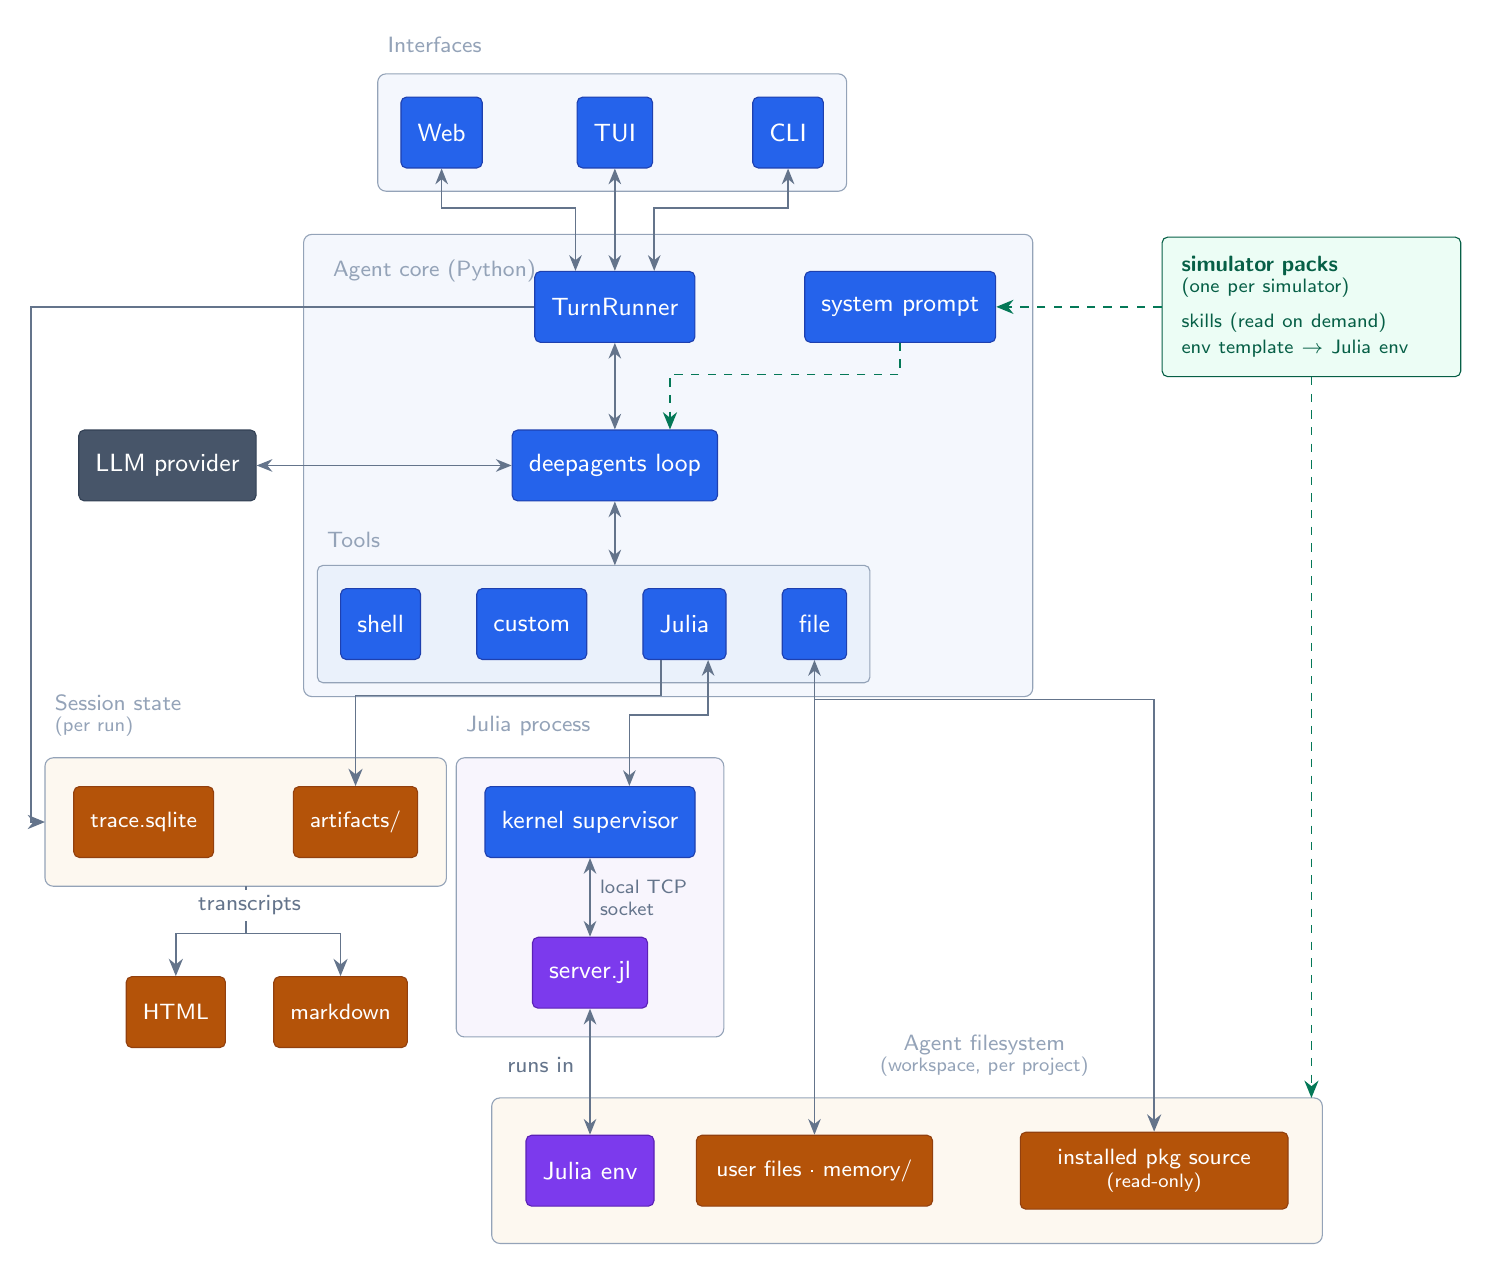
\begin{tikzpicture}

  % ===== agent core spine, interfaces centred over the TurnRunner =====
  \node[python] (runner) {TurnRunner};
  \node[python, anchor=south] (web) at ([xshift=-22mm,yshift=13mm]runner.north) {Web};
  \node[python, anchor=south] (tui) at ([yshift=13mm]runner.north) {TUI};
  \node[python, anchor=south] (cli) at ([xshift=22mm,yshift=13mm]runner.north) {CLI};

  \node[python, below=11mm of runner] (loop) {deepagents loop};

  % tools row, centred under the loop
  \node[python, anchor=north east] (ct) at ([xshift=-3.5mm,yshift=-11mm]loop.south) {custom};
  \node[python, left=7mm of ct] (sh) {shell};
  \node[python, anchor=north west] (jt) at ([xshift=3.5mm,yshift=-11mm]loop.south) {Julia};
  \node[python, right=7mm of jt] (ft) {file};

  % ===== prompt inside the core, packs beside it, LLM on the left =====
  \node[python] (prompt) at ([xshift=26mm]runner.east |- runner) {system prompt};
  \node[external, anchor=east] (llm) at ([xshift=-10.6mm]sh.west |- loop) {LLM provider};
  \node[data, anchor=west, text width=33mm] (pack) at ([xshift=21mm]prompt.east) {%
    \textbf{simulator packs}\\[-2pt]
    {\scriptsize (one per simulator)}\\[3pt]
    {\scriptsize skills (read on demand)}\\
    {\scriptsize env template $\rightarrow$ Julia env}};

  % ===== left column: session state =====
  \node[storage, below left=16mm and 16mm of sh] (trace) {trace.sqlite};
  \node[storage, right=10mm of trace] (arts) {artifacts/};
  \coordinate (sessmid) at ($(trace.south)!0.5!(arts.south)$);
  \node[storage, anchor=north east] (html) at ([xshift=-3mm,yshift=-15mm]sessmid) {HTML};
  \node[storage, anchor=north west] (md) at ([xshift=3mm,yshift=-15mm]sessmid) {markdown};

  % ===== julia process column, left of the file-tool feed =====
  \node[python, below=16mm of jt, xshift=-12mm] (kern) {kernel supervisor};
  \node[julia, below=10mm of kern] (serv) {server.jl};

  % ===== bottom: filesystem; env straight under the server =====
  \node[julia, anchor=north] (env) at ([yshift=-16mm]serv.south) {Julia env};
  \node[storage, minimum width=30mm] (files) at (ft |- env) {user files · memory/};
  \node[storage, right=11mm of files, minimum width=34mm] (mounts) {%
    installed pkg source\\[-1pt]
    {\scriptsize (read-only)}};

  % ===== group boxes =====
  \begin{scope}[on background layer]
    \node[fit=(web)(tui)(cli), inner sep=8pt] (ifacebox) {};
    \draw[jagroup, fill=jafillblue, rounded corners=3pt] (ifacebox.south west) rectangle (ifacebox.north east);
    \node[grouplabel, anchor=south west] at ([yshift=1.5mm]ifacebox.north west) {Interfaces};

    \node[fit=(runner)(loop)(sh)(ct)(jt)(ft)(prompt), inner sep=13pt] (corebox) {};
    \draw[jagroup, fill=jafillblue, rounded corners=3pt] (corebox.south west) rectangle (corebox.north east);
    \node[grouplabel, anchor=north west] at ([xshift=2.5mm,yshift=-2mm]corebox.north west) {Agent core (Python)};

    \node[fit=(sh)(ct)(jt)(ft), inner sep=8pt] (toolsbox) {};
    \draw[jagroup, fill=jafilltools, rounded corners=2pt] (toolsbox.south west) rectangle (toolsbox.north east);
    \node[grouplabel, anchor=south west] at ([yshift=1mm]toolsbox.north west) {Tools};

    \node[fit=(trace)(arts), inner sep=10pt] (sessbox) {};
    \draw[jagroup, fill=jafillamber, rounded corners=3pt] (sessbox.south west) rectangle (sessbox.north east);
    \node[grouplabel, anchor=south west, align=left] at ([yshift=1.5mm]sessbox.north west)
      {Session state\\[-2pt]{\scriptsize (per run)}};

    \node[fit=(kern)(serv), inner sep=10pt] (jlbox) {};
    \draw[jagroup, fill=jafillpurple, rounded corners=3pt] (jlbox.south west) rectangle (jlbox.north east);
    \node[grouplabel, anchor=south west] at ([yshift=1.5mm]jlbox.north west) {Julia process};

    \node[fit=(env)(files)(mounts), inner sep=12pt] (fsbox) {};
    \draw[jagroup, fill=jafillamber, rounded corners=3pt] (fsbox.south west) rectangle (fsbox.north east);
    \coordinate (fslabelx) at ($(files.north)!0.5!(mounts.north)$);
    \node[grouplabel, anchor=south, align=center] at ([yshift=1.5mm]fslabelx |- fsbox.north)
      {Agent filesystem\\[-2pt]{\scriptsize (workspace, per project)}};
  \end{scope}

  % ===== edges =====
  \draw[bi] (web.south) -- ++(0,-5mm) -| ([xshift=-5mm]runner.north);
  \draw[bi] (tui.south) -- ++(0,-5mm) -| (runner.north);
  \draw[bi] (cli.south) -- ++(0,-5mm) -| ([xshift=5mm]runner.north);
  \draw[bi] (runner.south) -- (loop.north);
  \draw[ard] (pack.west) -- (prompt.east);
  \draw[ard] (pack.south) -- (pack.south |- fsbox.north);
  \draw[ard] (prompt.south) -- ++(0,-4mm) -| ([xshift=7mm]loop.north);
  \draw[bi] (llm.east) -- (loop.west);
  \draw[bi] (loop.south) -- (loop.south |- toolsbox.north);

  % TurnRunner -> session state, dropping left of the LLM provider
  \coordinate (leftbus) at ($(llm.west)+(-6mm,0)$);
  \draw[ar] (runner.west) -- (leftbus |- runner.west) -- (leftbus |- sessbox.west) -- (sessbox.west);
  \draw[ar] (sessbox.south) -- ++(0,-6mm) -| (html.north);
  \draw[ar] (sessbox.south) -- ++(0,-6mm) -| (md.north);
  \node[el] at ([yshift=-6mm]sessmid) {transcripts};

  % julia spine and artifacts, on separate bands so nothing crosses
  \draw[bi] ([xshift=3mm]jt.south) -- ++(0,-7mm) -| ([xshift=5mm]kern.north);
  \draw[ar] ([xshift=-3mm]jt.south) -- ++(0,-4.5mm) -| (arts.north);
  \draw[bi] (kern.south) -- node[right, align=left, font=\scriptsize\sffamily, text=jasub] {local TCP\\socket} (serv.north);
  \draw[bi] (serv.south) -- node[el, left=1.2mm, pos=0.45] {runs in} (env.north);

  % file tool -> workspace nodes
  \draw[bi] (ft.south) -- (files.north);
  \draw[ar] ([yshift=-5mm]ft.south) -| (mounts.north);

\end{tikzpicture}
\end{document}
' && dvisvgm --no-fonts architecture.dvi -o architecture-dark.svg
\documentclass[tikz,border=32pt]{standalone}
\usepackage[T1]{fontenc}
\usepackage{lmodern}
\usepackage{xcolor}
\usetikzlibrary{positioning,fit,backgrounds,arrows.meta,calc}

\ifdefined\darkmode
  \definecolor{jafillblue}{RGB}{23,31,46}
  \definecolor{jafilltools}{RGB}{29,39,58}
  \definecolor{jafillamber}{RGB}{38,30,20}
  \definecolor{jafillpurple}{RGB}{32,26,46}
  \definecolor{jagroup}{RGB}{100,116,139}
  \definecolor{jaarrow}{RGB}{148,163,184}
  \definecolor{jadatabg}{RGB}{6,78,59}
  \definecolor{jadatatext}{RGB}{167,243,208}
  \definecolor{jasub}{RGB}{148,163,184}
  \definecolor{jalabelbg}{RGB}{30,41,59}
\else
  \definecolor{jafillblue}{RGB}{244,247,253}
  \definecolor{jafilltools}{RGB}{234,241,251}
  \definecolor{jafillamber}{RGB}{253,248,240}
  \definecolor{jafillpurple}{RGB}{248,245,253}
  \definecolor{jagroup}{RGB}{148,163,184}
  \definecolor{jaarrow}{RGB}{100,116,139}
  \definecolor{jadatabg}{RGB}{236,253,245}
  \definecolor{jadatatext}{RGB}{6,95,70}
  \definecolor{jasub}{RGB}{100,116,139}
  \definecolor{jalabelbg}{RGB}{255,255,255}
\fi

\definecolor{japython}{RGB}{37,99,235}
\definecolor{japythonstroke}{RGB}{30,64,175}
\definecolor{jajulia}{RGB}{124,58,237}
\definecolor{jajuliastroke}{RGB}{91,33,182}
\definecolor{jastorage}{RGB}{180,83,9}
\definecolor{jastoragestroke}{RGB}{146,64,14}
\definecolor{jadata}{RGB}{4,120,87}
\definecolor{jadatastroke}{RGB}{6,95,70}
\definecolor{jaexternal}{RGB}{71,85,105}
\definecolor{jaexternalstroke}{RGB}{51,65,85}

\tikzset{
  base/.style={
    draw, rounded corners=2pt, font=\small\sffamily,
    align=center, inner sep=6pt, minimum height=9mm, text=white
  },
  python/.style={base, fill=japython, draw=japythonstroke},
  julia/.style={base, fill=jajulia, draw=jajuliastroke},
  storage/.style={base, fill=jastorage, draw=jastoragestroke, font=\footnotesize\sffamily},
  external/.style={base, fill=jaexternal, draw=jaexternalstroke},
  data/.style={
    draw=jadatastroke, rounded corners=2pt, fill=jadatabg,
    font=\footnotesize\sffamily, align=left, inner sep=7pt, text=jadatatext
  },
  grouplabel/.style={font=\footnotesize\sffamily, text=jagroup},
  bi/.style={
    {Stealth[length=2mm,width=1.6mm]}-{Stealth[length=2mm,width=1.6mm]},
    draw=jaarrow, semithick
  },
  ar/.style={-{Stealth[length=2.2mm,width=1.8mm]}, draw=jaarrow, semithick},
  ard/.style={-{Stealth[length=2.2mm,width=1.8mm]}, draw=jadata, semithick, dashed},
  el/.style={font=\footnotesize\sffamily, text=jasub, fill=jalabelbg, inner sep=2pt},
}

\begin{document}
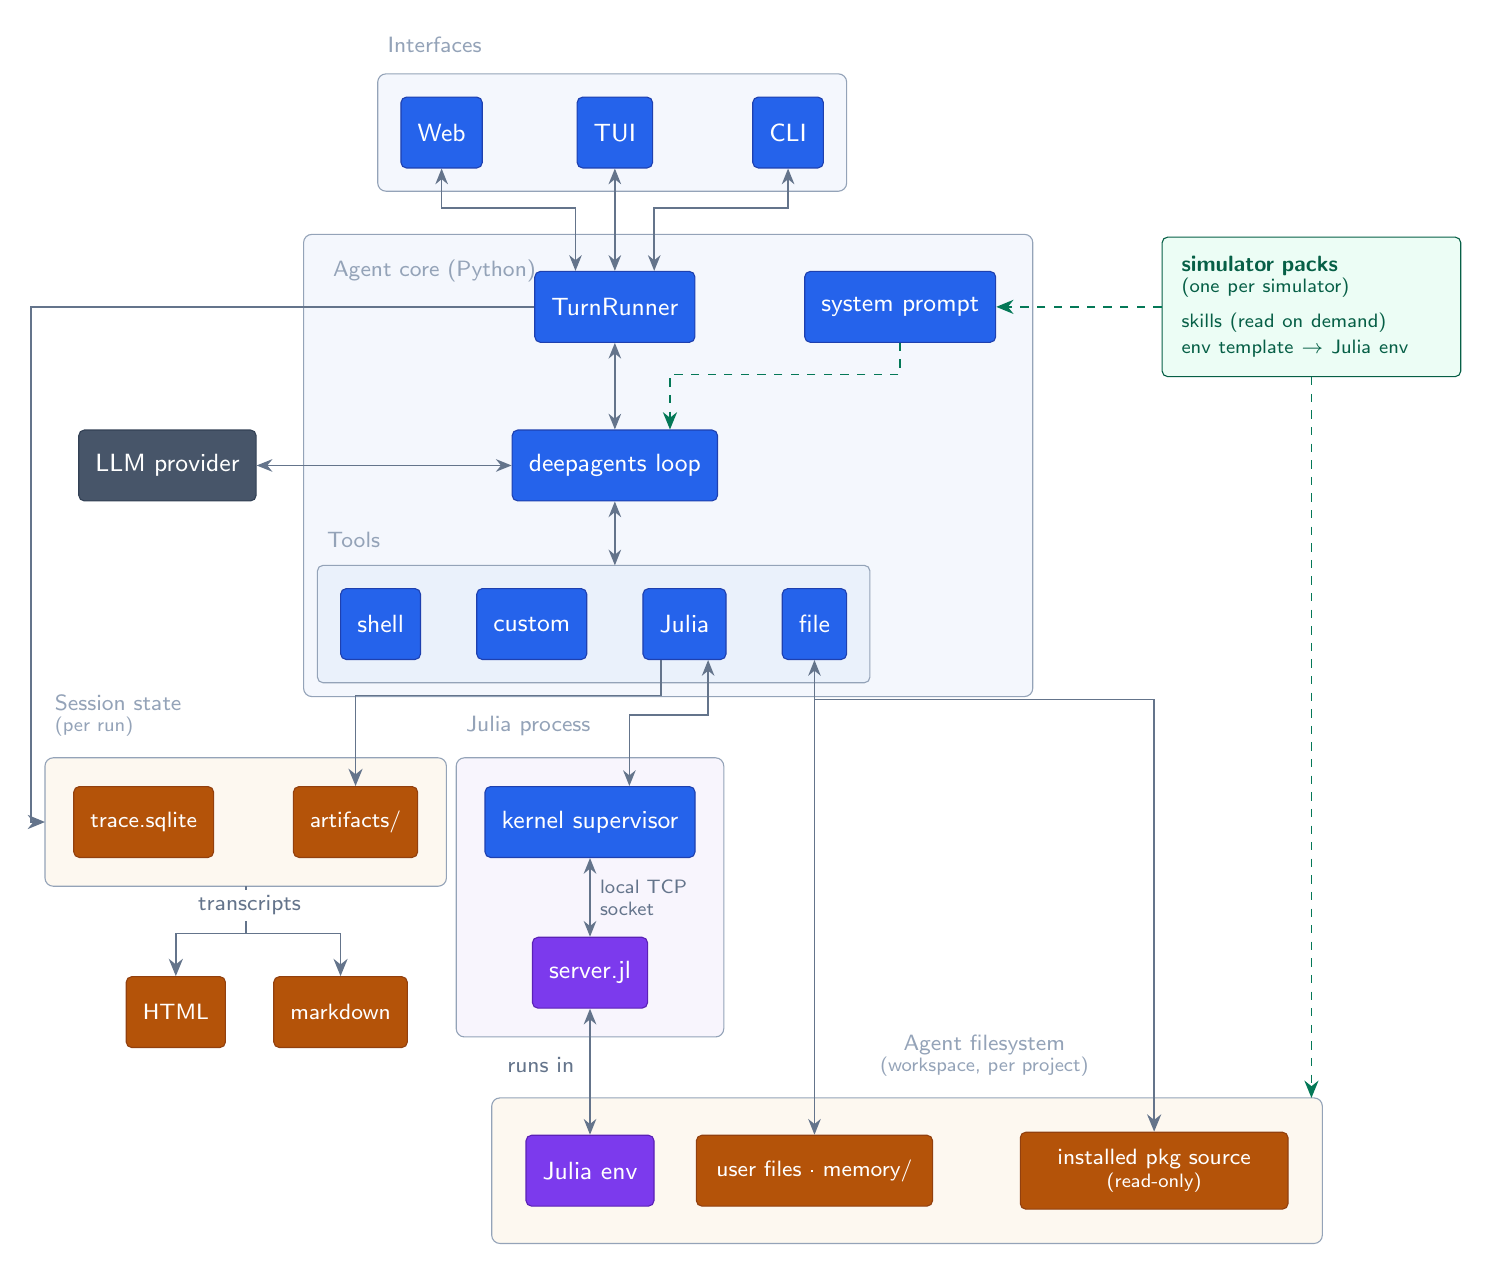
\begin{tikzpicture}

  % ===== agent core spine, interfaces centred over the TurnRunner =====
  \node[python] (runner) {TurnRunner};
  \node[python, anchor=south] (web) at ([xshift=-22mm,yshift=13mm]runner.north) {Web};
  \node[python, anchor=south] (tui) at ([yshift=13mm]runner.north) {TUI};
  \node[python, anchor=south] (cli) at ([xshift=22mm,yshift=13mm]runner.north) {CLI};

  \node[python, below=11mm of runner] (loop) {deepagents loop};

  % tools row, centred under the loop
  \node[python, anchor=north east] (ct) at ([xshift=-3.5mm,yshift=-11mm]loop.south) {custom};
  \node[python, left=7mm of ct] (sh) {shell};
  \node[python, anchor=north west] (jt) at ([xshift=3.5mm,yshift=-11mm]loop.south) {Julia};
  \node[python, right=7mm of jt] (ft) {file};

  % ===== prompt inside the core, packs beside it, LLM on the left =====
  \node[python] (prompt) at ([xshift=26mm]runner.east |- runner) {system prompt};
  \node[external, anchor=east] (llm) at ([xshift=-10.6mm]sh.west |- loop) {LLM provider};
  \node[data, anchor=west, text width=33mm] (pack) at ([xshift=21mm]prompt.east) {%
    \textbf{simulator packs}\\[-2pt]
    {\scriptsize (one per simulator)}\\[3pt]
    {\scriptsize skills (read on demand)}\\
    {\scriptsize env template $\rightarrow$ Julia env}};

  % ===== left column: session state =====
  \node[storage, below left=16mm and 16mm of sh] (trace) {trace.sqlite};
  \node[storage, right=10mm of trace] (arts) {artifacts/};
  \coordinate (sessmid) at ($(trace.south)!0.5!(arts.south)$);
  \node[storage, anchor=north east] (html) at ([xshift=-3mm,yshift=-15mm]sessmid) {HTML};
  \node[storage, anchor=north west] (md) at ([xshift=3mm,yshift=-15mm]sessmid) {markdown};

  % ===== julia process column, left of the file-tool feed =====
  \node[python, below=16mm of jt, xshift=-12mm] (kern) {kernel supervisor};
  \node[julia, below=10mm of kern] (serv) {server.jl};

  % ===== bottom: filesystem; env straight under the server =====
  \node[julia, anchor=north] (env) at ([yshift=-16mm]serv.south) {Julia env};
  \node[storage, minimum width=30mm] (files) at (ft |- env) {user files · memory/};
  \node[storage, right=11mm of files, minimum width=34mm] (mounts) {%
    installed pkg source\\[-1pt]
    {\scriptsize (read-only)}};

  % ===== group boxes =====
  \begin{scope}[on background layer]
    \node[fit=(web)(tui)(cli), inner sep=8pt] (ifacebox) {};
    \draw[jagroup, fill=jafillblue, rounded corners=3pt] (ifacebox.south west) rectangle (ifacebox.north east);
    \node[grouplabel, anchor=south west] at ([yshift=1.5mm]ifacebox.north west) {Interfaces};

    \node[fit=(runner)(loop)(sh)(ct)(jt)(ft)(prompt), inner sep=13pt] (corebox) {};
    \draw[jagroup, fill=jafillblue, rounded corners=3pt] (corebox.south west) rectangle (corebox.north east);
    \node[grouplabel, anchor=north west] at ([xshift=2.5mm,yshift=-2mm]corebox.north west) {Agent core (Python)};

    \node[fit=(sh)(ct)(jt)(ft), inner sep=8pt] (toolsbox) {};
    \draw[jagroup, fill=jafilltools, rounded corners=2pt] (toolsbox.south west) rectangle (toolsbox.north east);
    \node[grouplabel, anchor=south west] at ([yshift=1mm]toolsbox.north west) {Tools};

    \node[fit=(trace)(arts), inner sep=10pt] (sessbox) {};
    \draw[jagroup, fill=jafillamber, rounded corners=3pt] (sessbox.south west) rectangle (sessbox.north east);
    \node[grouplabel, anchor=south west, align=left] at ([yshift=1.5mm]sessbox.north west)
      {Session state\\[-2pt]{\scriptsize (per run)}};

    \node[fit=(kern)(serv), inner sep=10pt] (jlbox) {};
    \draw[jagroup, fill=jafillpurple, rounded corners=3pt] (jlbox.south west) rectangle (jlbox.north east);
    \node[grouplabel, anchor=south west] at ([yshift=1.5mm]jlbox.north west) {Julia process};

    \node[fit=(env)(files)(mounts), inner sep=12pt] (fsbox) {};
    \draw[jagroup, fill=jafillamber, rounded corners=3pt] (fsbox.south west) rectangle (fsbox.north east);
    \coordinate (fslabelx) at ($(files.north)!0.5!(mounts.north)$);
    \node[grouplabel, anchor=south, align=center] at ([yshift=1.5mm]fslabelx |- fsbox.north)
      {Agent filesystem\\[-2pt]{\scriptsize (workspace, per project)}};
  \end{scope}

  % ===== edges =====
  \draw[bi] (web.south) -- ++(0,-5mm) -| ([xshift=-5mm]runner.north);
  \draw[bi] (tui.south) -- ++(0,-5mm) -| (runner.north);
  \draw[bi] (cli.south) -- ++(0,-5mm) -| ([xshift=5mm]runner.north);
  \draw[bi] (runner.south) -- (loop.north);
  \draw[ard] (pack.west) -- (prompt.east);
  \draw[ard] (pack.south) -- (pack.south |- fsbox.north);
  \draw[ard] (prompt.south) -- ++(0,-4mm) -| ([xshift=7mm]loop.north);
  \draw[bi] (llm.east) -- (loop.west);
  \draw[bi] (loop.south) -- (loop.south |- toolsbox.north);

  % TurnRunner -> session state, dropping left of the LLM provider
  \coordinate (leftbus) at ($(llm.west)+(-6mm,0)$);
  \draw[ar] (runner.west) -- (leftbus |- runner.west) -- (leftbus |- sessbox.west) -- (sessbox.west);
  \draw[ar] (sessbox.south) -- ++(0,-6mm) -| (html.north);
  \draw[ar] (sessbox.south) -- ++(0,-6mm) -| (md.north);
  \node[el] at ([yshift=-6mm]sessmid) {transcripts};

  % julia spine and artifacts, on separate bands so nothing crosses
  \draw[bi] ([xshift=3mm]jt.south) -- ++(0,-7mm) -| ([xshift=5mm]kern.north);
  \draw[ar] ([xshift=-3mm]jt.south) -- ++(0,-4.5mm) -| (arts.north);
  \draw[bi] (kern.south) -- node[right, align=left, font=\scriptsize\sffamily, text=jasub] {local TCP\\socket} (serv.north);
  \draw[bi] (serv.south) -- node[el, left=1.2mm, pos=0.45] {runs in} (env.north);

  % file tool -> workspace nodes
  \draw[bi] (ft.south) -- (files.north);
  \draw[ar] ([yshift=-5mm]ft.south) -| (mounts.north);

\end{tikzpicture}
\end{document}
